%%%%%%%%%%%%%%%%%%%%%%%%%%%%%%%%%%%%%%%%%%%%%%%%%%%%%%%%%%%%%%%%%%%%%%%%%%%%%%%
\section{Get involved!}
\label{sec:getinvolved}
%%%%%%%%%%%%%%%%%%%%%%%%%%%%%%%%%%%%%%%%%%%%%%%%%%%%%%%%%%%%%%%%%%%%%%%%%%%%%%%
So you want to help look for magnetic monopoles at the Large Hadron Collider?
Great! This section will take you through what you need to do, how to do it,
and how to get help if you need it.

%=============================================================================
\subsection{Getting started}
\label{sec:zooniversegettingstarted}
%=============================================================================
In order to give you access to the MoEDAL experiment data,
and tools you'll need to analyse it, the Institute for Research in Schools
has called in some help from our friends at the
\href{http://www.zooniverse.org}{Zooniverse}.
The Zooniverse started with the
\href{http://www.galaxyzoo.org}{Galaxy Zoo} project,
where people were invited to classify thousands of images of galaxies from
the Sloan Digital Sky Survey.
It has since evolved into the world's largest and most popular platform
for people-powered research that has led to peer-reviewed publications
and opened the door to many new areas of scientific research that just
would not be possible otherwise.
MoEDAL has created the Monopole Quest! project within the Zooniverse,
and by taking part in this you'll be joining the millions of Zooniverse
volunteers helping to do
\href{https://www.zooniverse.org/about/publications}{real science}.

%-----------------------------------------------------------------------------
\subsubsection{Creating a Zooniverse account}
\label{sec:zooniverseaccount}
%-----------------------------------------------------------------------------
The first thing to do is to visit the Zooniverse website\footnote{%
See \href{http://www.zooniverse.org}{http://www.zooniverse.org}}
and create a user account.
%
You can do this on a desktop computer, a laptop, a tablet or even a
smartphone (if the screen is big enough!).
If you're a student, you may wish to ask your teacher to do this for you
or for them to create an account for your class.
You don't have to create an account to take part in Monopole Quest!,
but in order for your work to be credited you need to be logged in.
Always ask your teacher or your IRIS contact for advice if you need to.
Creating a user account is simple -- you can create a user account by
filling in the online form you get when you click on the ``Register''
link at the top-right of the Zooniverse homepage.

%-----------------------------------------------------------------------------
\subsubsection{Sign in and access the Monopole Quest! project}
\label{sec:zooniversesignin}
%-----------------------------------------------------------------------------
Once you have created an account,
sign in to the Zooniverse by clicking the ``Sign in'' link
(also at the top-right of the homepage).
Then you can access the Monopole Quest! project at the following URL:

\begin{itemize}
\item \url{https://www.zooniverse.org/projects/twhyntie/monopole-quest}
\end{itemize}

After which you should see the Monopole Quest! landing page as
shown in Figure~\ref{fig:mqlandingpage}.

%
\begin{figure}[htbp]
  \centering
  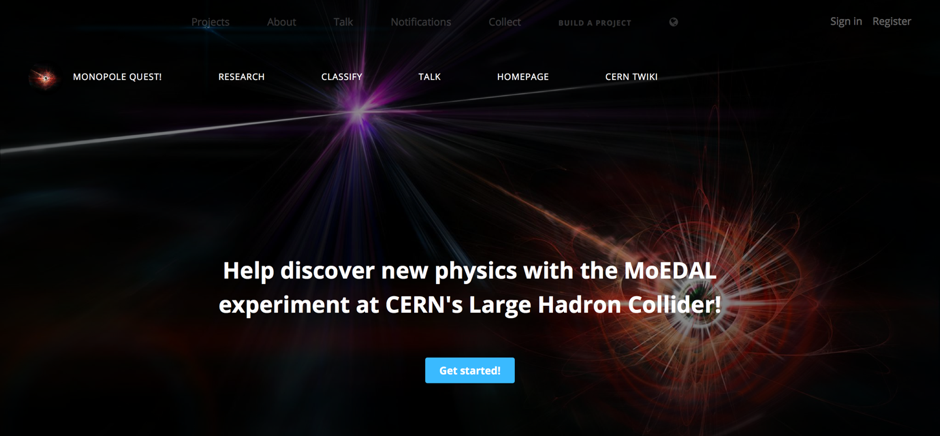
\includegraphics[width=1.0\textwidth]{assets/images/mqlandingpage/mqlandingpage.png}
  \caption[The Monopole Quest! project landing page]
  {\label{fig:mqlandingpage}The Monopole Quest! landing page on the Zooniverse.
From here you can get stuck into some real MoEDAL data straight away!}
\end{figure}
%

Then click on the ``Get started!'' button and start doing some science!

%=============================================================================
\subsection{The Monopole Quest! project}
\label{sec:monopolequest}
%=============================================================================

%-----------------------------------------------------------------------------
\subsubsection{What do I do?}
\label{sec:mqwhatdoido}
%-----------------------------------------------------------------------------
As with all Zooniverse projects, Monopole Quest! will ask you a number of
questions about an image from one or more their datasets.
Your answers to these questions will result in a classification for that
image -- information about that data that will help scientists with
some aspect of the research.
For example, the first question in Monopole Quest! asks you if you can
see any ``blobs'' in the image (see Figure~\ref{fig:mqblobq}).
These blobs correspond to the etched pits in the
\ac{NTD} scans that may be caused by monopoles or other \acp{HIP}.
So, in essence, you are being asked if you can see any potential
monopole signals!

You can answer the questions by selecting the appropriate answer with your
mouse (or tapping the option on a touch screen) and then pressing the
``Done'' button.
You'll then be asked the next question or asked to perform a task,
such as drawing a shape on the image.
For example, if you can see a blob in the image, you'll be asked to draw
around it with a circle (the ``blob marking tool'') in order to measure
its size (see Figure~\ref{fig:mqdrawing}).

%
\begin{figure}[p]
  \centering
  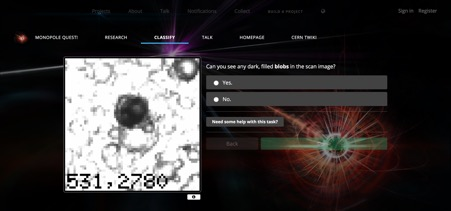
\includegraphics[width=0.8\textwidth]{assets/images/mqblobq/mqblobq.jpg}
  \caption[Monopole Quest! Can you see any blobs?]
  {\label{fig:mqblobq}The first question from the Monopole Quest!
Zooniverse project (Jan. 2017).}
\end{figure}
%

%
\begin{figure}[p]
  \centering
  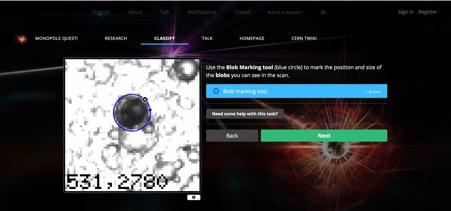
\includegraphics[width=0.8\textwidth]{assets/images/mqdrawing/mqdrawing.jpg}
  \caption[Monopole Quest! An example drawing task]
  {\label{fig:mqdrawing}An example drawing task in the Monopole Quest! project
(Jan. 2017).}
\end{figure}
%

%-----------------------------------------------------------------------------
\subsubsection{How do I get help?}
\label{sec:mqhelp}
%-----------------------------------------------------------------------------
As there are many questions and tasks to do in Monopole Quest!,
we have added interactive help to the questions themselves rather than
list everything here.  If you need help at any point, click on the
``Need some help with this task?'' button and a pop-up window will appear
that will give you some additional guidance if you get stuck.
Figure~\ref{fig:mqhelp} shows an example of this.

%
\begin{figure}[htbp]
  \centering
  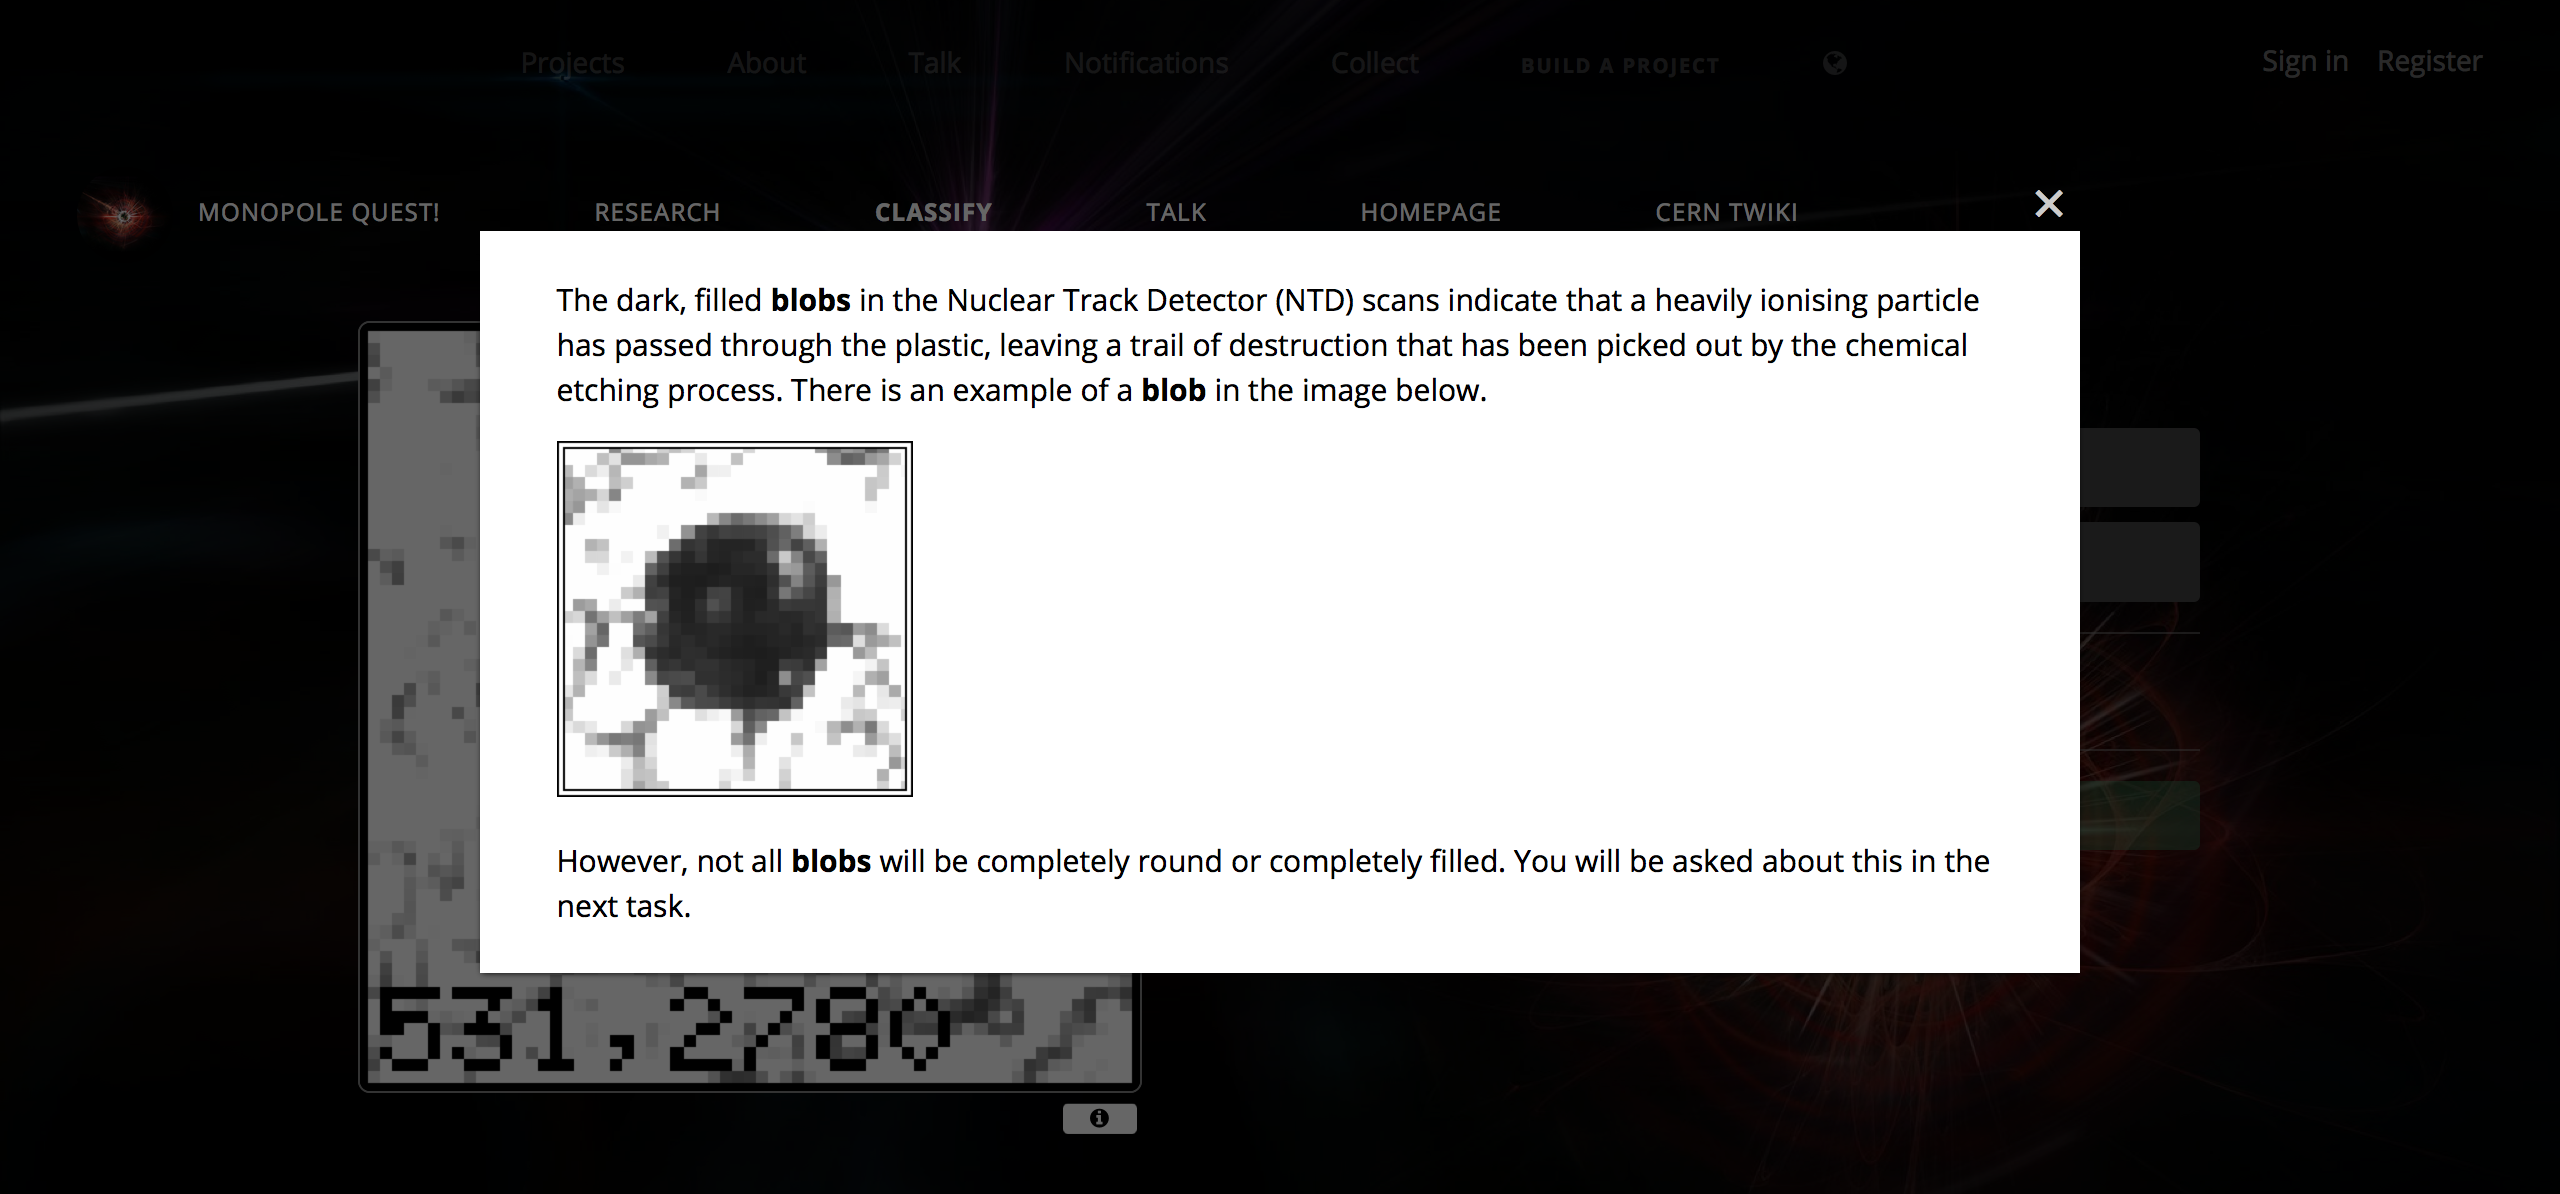
\includegraphics[width=0.8\textwidth]{assets/images/mqhelp/mqhelp.png}
  \caption[Monopole Quest! An example help message]
  {\label{fig:mqhelp}An example help pop-up message in Monopole Quest! (Jan. 2017).}
\end{figure}
%

\clearpage

%-----------------------------------------------------------------------------
\subsubsection{What am I looking at?}
\label{sec:mqlookingat}
%-----------------------------------------------------------------------------
The data used in Monopole Quest! comes from scans of plastic from the
\ac{MoEDAL} \acp{NTD}.
All of it is real data from the experiment,
but some images were made using plastic exposed to different environments
and scanned in different laboratories:

\begin{enumerate}
\item Some plastic was exposed to LHC collisions at 8 TeV centre-of-mass energy;
\item Some plastic was exposed to LHC collisions at 13 TeV centre-of mass energy;
\item Some plastic was exposed to a heavy ion test beam
(see Figure~\ref{fig:bnltestbeam});
\item Some plastic was exposed to both LHC collisions and a heavy ion test beam.
\end{enumerate}

%
\begin{figure}[htbp]
  \centering
  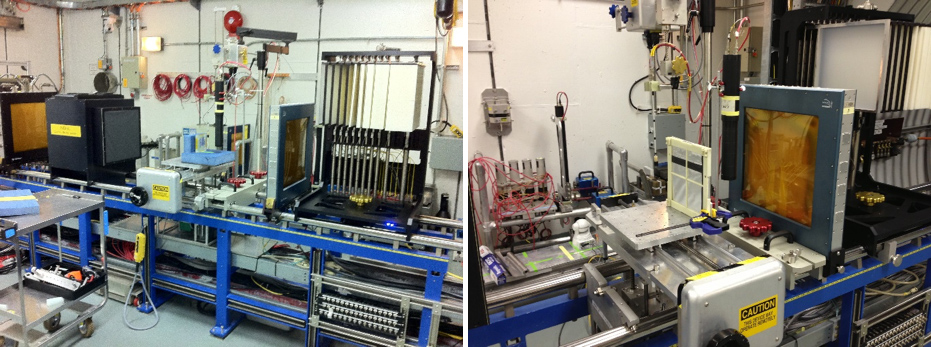
\includegraphics[width=1.0\textwidth]{assets/images/bnltestbeam/bnltestbeam.jpg}
  \caption[MoEDAL NTD samples in the BNL test beam]
  {\label{fig:bnltestbeam}\ac{MoEDAL} \ac{NTD} samples being exposed to a
heavy ion test beam at the \ac{NASA} \acf{SRL}, \acf{BNL}.
Exposing \ac{NTD} plastic to heavy ions from test beams allows us to see
what monopole-like signals might look like and put our analysis procedures
through their paces.  %
Image credit: R. Soluk/the MoEDAL Collaboration; %
please contact them regarding licensing/re-use of this image.}
\end{figure}
%

Analysis of plastic exposed to these different conditions is necessary to
provide control samples and to test our analysis procedures
(including Monopole Quest!) with monopole-like signals from the heavy ions.
As a Zooniverse volunteer, we won’t tell you which sample type you are 
looking at (as this might bias your answers).
However, all data and classifications are useful to the \ac{MoEDAL}
science programme, so please do as many as you can!

%-----------------------------------------------------------------------------
\subsubsection{What happens next? Continuing your MoEDAL journey}
\label{sec:mqnext}
%-----------------------------------------------------------------------------
Your classifications are stored by Monopole Quest! for further analysis
by the \ac{MoEDAL} science team -- which could include you!
As you and your school get further involved with \ac{IRIS},
data based on the user classifications (including yours) can be made 
available for individual or group research projects.
Contact the \ac{IRIS} team with your Zooniverse usernames
(so we can verify how many classifications you have made)
and project ideas to find out more.
Then, as with all \ac{IRIS} research,
the aim is to publish results based on the data and analysis in
peer-reviewed scientific journals.
You can see the many examples of Zooniverse-powered publications on their
website -- and with the support of CERN@school through IRIS
and the MoEDAL Collaboration, you should be able to add to this.

{\color{white}Spacer}
\\[1cm]

\begin{center}
\textbf{What can {\em you} do with \ac{MoEDAL} and \ac{IRIS}?}
\end{center}
